\documentclass[12pt,twoside,a4paper]{article} 
%\includeonly{1D_spectra}


%--- Packages to use
%
%\usepackage{scrpage}
\usepackage[latin1]{inputenc}
\usepackage[]{fancyhdr}   
\usepackage[]{natbib}
\usepackage{alltt}
\usepackage{mathptmx}
\usepackage{verbatim}
\usepackage{lscape}         % landscape mode of a single page
\usepackage[]{longtable}    % allow tables longer than one page
%\usepackage{makeidx}        % index of terms
\usepackage{tabularx}       % allows line breaking in table columns
%\usepackage{algorithm}      % for describing algorithms with pseudo-code
%\usepackage{algorithmic}
%\usepackage{ifthen}
\usepackage{url}
\usepackage{amsfonts}

\raggedbottom



%% Nimm die Seitennummern nach oben:
%\renewpagestyle{plain}{(0pt,0pt)%     Head
%                       {\hfill}{\hfill}{\hfill}%
%                       (0pt,0pt)}%
%                      {(0pt,0pt)%     Foot
%                       {\hfill}{\hfill}{\hfill}%
%                       (0pt,0pt)}
%\renewpagestyle{headings}{(0pt,0pt)%
%%                          {\pagemark \hspace{1cm} \leftmark\hfill}%
%%                          {\hfill\rightmark \hspace{1cm} \pagemark}%
%                          {\pagemark\hfill\leftmark}%
%                          {\rightmark\hfill\pagemark}%
%                          {\hfill\headmark \pagemark}%
%                          (0pt,0pt)}%
%                         {(0pt,0pt)%
%                          {\hfill}{\hfill}{\hfill}%
%                          (0pt,0pt)}
% 

%%% Din A4 paper, as draft for review
%\hoffset-1in
%\voffset-1in
%%\addtolength{\voffset}{0.4cm}
%
\oddsidemargin0.5cm
\evensidemargin0.5cm
\textwidth15cm
%\topmargin3cm           % = 4cm on top of page
%\headheight1cm
%\headsep1cm
%
\textheight22cm         % = 4c
\parindent0cm

\pagestyle{fancy}
\fancyhf{}
\fancyhead[LE,RO]{\bfseries \thepage}
\fancyhead[LO]{\bfseries \rightmark}
\fancyhead[RE]{\bfseries \leftmark}
\renewcommand{\headrulewidth}{0pt} 

%
%--- Some layout commands
%
\sloppy
\raggedbottom
\hbadness=10000
\bibliographystyle{agu}

%
%--- PDF
%
\DeclareGraphicsExtensions{.pdf}
\usepackage{color}
\usepackage
[pdftex,                         % or dvips
a4paper,
linktocpage,
colorlinks=true,
pdftitle={Monte Carlo Method for Radiative Transfer},
pdfauthor={Claudia Emde <claudia.emde@dlr.de>},
pdfsubject={},
pdfkeywords={Claudia Emde, radiative transfer, Monte Carlo},
bookmarks=true,
bookmarksopen=true,
bookmarksnumbered,
pdfpagemode=UseOutlines
%pdfpagemode=None,
%plainpages=false,
%pdfpagelabels
]{hyperref}

\usepackage[pdftex]{graphicx} 
\setcounter{tocdepth}{3}

\hyphenation{}

% Differential d
\newcommand{\DiffD}         {\ensuremath{\mathrm{d}}}
% =======================================================================
% ***************************** Begin Document **************************
% =======================================================================
\begin{document}

%\frontmatter


\title{Atmospheric radiative transfer modeling using the \\Monte Carlo method}
\author{Claudia Emde\\
  Ludwig-Maximilians-Universit{\"a}t (LMU) \\
  Munich, Germany}

\date{April 2010}

\maketitle
                                
\pagestyle{headings}

\newpage 

\tableofcontents

\cleardoublepage
\section{Simulation of random variables} 
\label{sec:random_numbers}

Assume that a continous random variable $\xi$ is defined by its probability 
density function p(x), defined on the interval $x_{min} \le x \le
x_{max}$. The normalized cumulative distribution $F(x)$ is defined as 
\begin{equation}
  F(x)=\frac{\int_{x_\mathrm{min}}^{x} p(x') dx'}{\int_{x_\mathrm{min}}^{x_\mathrm{max}} p(x') dx'}
\end{equation}
If we want to generate a sample of random numbers which are
distributed according to $p(x)$, we may use a random number generator
that produces uniformly distributed random numbers $r$
between 0 and 1 and solve 
\begin{equation}
  F(\xi)=r
\end{equation}
Inversion of $F$ gives
\begin{equation}
  \xi=F^{-1}(r)
\end{equation}

\subsection{Rayleigh phase function}

The scattering phase function can be interpreted as the probablity
density function for the scattering direction. 
 
If the particles are small compared to the wavelength of the
radiation (Rayleigh scattering), the phase function $P_\mathrm{R}$ is 
\begin{equation}
  P_\mathrm{R}(\theta) = \frac{3}{4}(1+\cos^2\theta)
\end{equation}
or with $\mu=\cos\theta$
\begin{equation}
  P_\mathrm{R}(\mu) = \frac{3}{4}(1+\mu^2)
\end{equation}
Here $\theta$ is the scattering angle. 
Scattering of solar radiation in the atmosphere by molecules is
described by Rayleigh scattering.

In order to calculate a random sample of scattering angles we have to solve
\begin{equation}
  r= F(\mu) = \frac{\int_{-1}^{\mu} \frac{3}{4}(1+\mu'^2) \DiffD\mu'}
  {\int_{-1}^{1} \frac{3}{4}(1+\mu'^2) \DiffD\mu'}
\end{equation}
This yields the following cubic equation: 
\begin{equation}
  \label{eq:rayleigh_cubic}
  \mu^3 + 3\mu - 8 r + 4 = 0
\end{equation}
The solution of a cubic equation is given by Cardano's formula. 
\begin{equation}
  \mu = u - 1/u
\end{equation}
with 
\begin{eqnarray}
  u =& (-q/2 + \sqrt{D})^{1/3}\\
  q =& -8 r + 4\\
  D =& 1 + q^2/4
\end{eqnarray}
Figure \ref{fig:rayleigh} shows the Rayleigh phase function,
the integated (cumulative) phase
function and a histogram of randomly sampled $\mu$-values.
\begin{figure}[b!]
  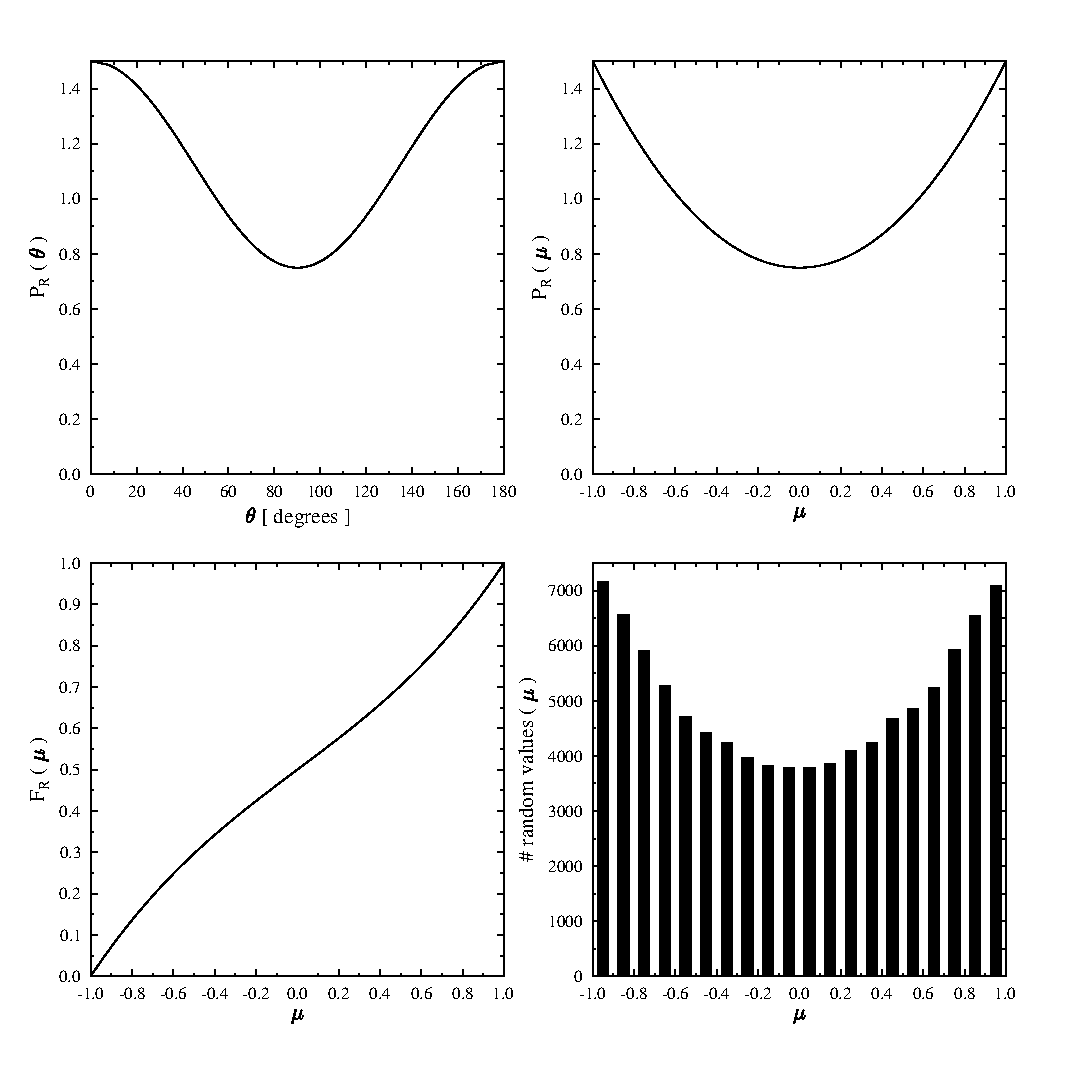
\includegraphics[width=0.9\hsize]{../examples/rayleigh.pdf}
  \caption{Top left: $P_\mathrm{R}$ as a function of the scattering angle $\theta$. Top right: $P_R$ as a function of the cosine of the scattering angle $\mu=cos(\theta)$. Bottom left: Cumulative probability density function for Rayleigh scattering. Bottom right: Histogram of randomly sampled values of $\mu$ using 100.000 random numbers.} 
  \label{fig:rayleigh}
\end{figure}

\subsection{Henyey-Greenstein phase function}

For larger particles in the atmosphere like cloud droplets/particles or
aerosols the scattering phase functions can be rather complex (see
Fig. \ref{fig:phase_functions}).
An analytical approximative fit for this kind of phase
functions has been proposed by \citet{henyey41}:
\begin{equation}
  \label{eq:henyey_greenstein}
  P_\mathrm{HG}(\mu)=\frac{1-g^2}{(1+g^2-2g\mu)^{3/2}}
\end{equation}
Here $g$ is the asymmetry parameter which describes the
distribution of forward and backward scattering. 
$g\rightarrow1$ means complete forward scattering, 
$g=0$ means isotropic scattering and for $g=-1$ we have complete
backward scattering.   
\begin{figure}[htbp]
  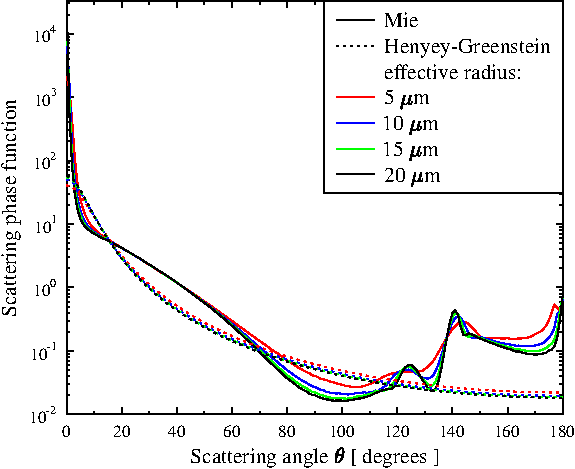
\includegraphics[width=.5\hsize]{./figs/phase_functions_water}
  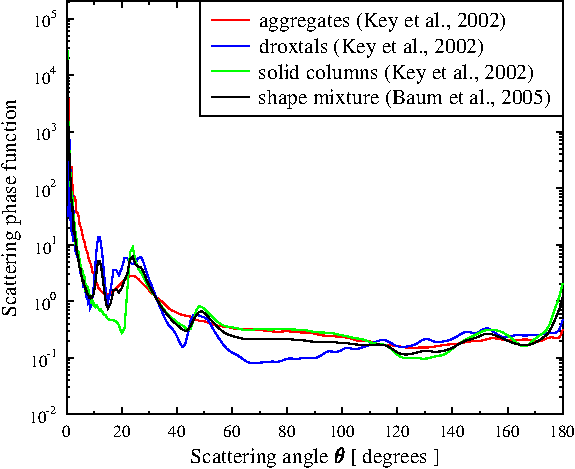
\includegraphics[width=.5\hsize]{./figs/phase_functions_ice}
  \caption{(Left) Mie scattering phase functions for water clouds with
    effective radii 5, 10, 15, and 20~$\mu$m (solid lines). Also shown are
    the respective Henyey-Greenstein approximations for the four
    cases, as provided by the parameterization of \citet{Hu93} (dashed lines).
    (Right) Ice cloud scattering phase
    functions for an effective radius of 50$\mu$m using different
    parameterizations; (red) parameterization by \citet{key2002} for rough
    aggregates; (blue) same but for droxtals; (green) same for solid columns,
    (black) parameterization by \citet{baum05b:_bulk}; the figure shows the
    typical behaviour of non-spherical particles, in particular the
    large difference in the sideward scattering direction compared to
    spherical particles.}
  \label{fig:phase_functions}
\end{figure}

\subsection{Optical thickness and photon path}

The distance $s$ that a photon travels between two interactions
with the medium is related to the optical thickness of the
medium. However, theoretically it is possible that the photon reaches the
surface without any interactions, even if the medium has a very
large optical thickness. 

The transmission $T$ is defined as
\begin{equation}
  T=\exp({-\int_{0}^{s} \beta_\mathrm{ext} ds'})=\exp({-\tau})
\end{equation}
where $\beta_\mathrm{ext}$ is the extinction coefficient, $s$ the distance
and $\tau$ the optical thickness. The transmission may be interpreted as the
probabily that the photon travels the distance $\tau$ without
interactions:
\begin{equation}
  P(\tau)=\exp(-\tau) 
\end{equation}

\subsection{Surface reflection}
\label{sec:surface}
The reflection of most surfaces depends on the incoming direction of
the photon as well as on the direction of the reflection. This is
modeled using Bidirectional Reflectance Distribution Functions
(BRDFs). There are simpler approximations, for instance the 
Lambertian reflection. Lambert's cosine law says that the radiant intensity
observed from a ``Lambertian'' surface is proportional to the cosine
of the angle $\theta$ between the observer's line of sight and the
surface normal. This means that when a surface is viewed from any
angle it has the same apparent radiance (see Fig.: \ref{fig:Lambert}).
\begin{figure}[htbp]
  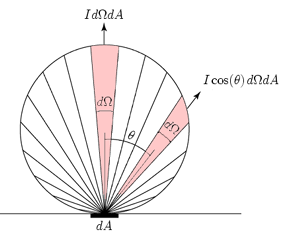
\includegraphics[width=.5\hsize]{./figs/LambertCosineLaw1.png}
  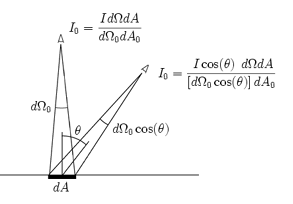
\includegraphics[width=.5\hsize]{./figs/LambertCosineLaw2.png}
  \caption{ Illustration of a Lambertian surface: (Left) Emission/reflection in normal and off-normal direction. (Right) Observed intensity for a normal and off-normal observer; $dA_0$ is the area of the observing aperture and d$\Omega_0$ is the solid angle subtended by the aperture from the viewpoint of the emitting area element. Source: Wikipedia.}
    \label{fig:Lambert}
\end{figure}

The probability distribution for the reflected direction of a Lambertian
surface is given by: 
\begin{equation}
  \label{eq:lambert}
  p(\theta)=\cos\theta  
\end{equation}


\subsection{Tasks}

\begin{enumerate}
\item Verify Eq.~\ref{eq:rayleigh_cubic}. Write a function that
  generates random scattering angles for Rayleigh scattering and
  reproduce Fig.~\ref{fig:rayleigh}.
\item Plot the Henyey-Greenstein phase function for various asymmetry 
  parameters.\\ 
  Generate random values of scattering angles for an asymmetry
  parameter of 0.85 (typical value for water clouds). 
\item Generate random values of optical thickness
  $\tau$ corresponding to the distance $s$ that a photon travels without
  interaction with the scattering medium. 
\item Generate random values of the reflection direction by a
  Lambertian surface.

Verify the results by plotting histograms of the sampled random numbers.

\end{enumerate}

\cleardoublepage

\section{Cloud scattering}
\label{sec:clouds}

\subsection{Setup: Homogeneous cloud layer}

We would like to calculate the transmittance and reflectance of a
homogeneous horizontally infinite cloud layer. We make the following
assumptions: The geometrical thickness of the cloud layer is $\Delta z$. The
scattering of the cloud droplets can be described by a
Henyey-Greenstein phase function with asymmetry parameter $g$.  
The vertical optical thickness of the cloud layer is
$\tau_c=\beta_{ext} \Delta z$. We assume that there is 
no absorption, i.e., energy is conserved. This simple setup is depicted in
Fig.\ref{fig:cloudonly}. 

\begin{figure}[htbp]
  \centering
  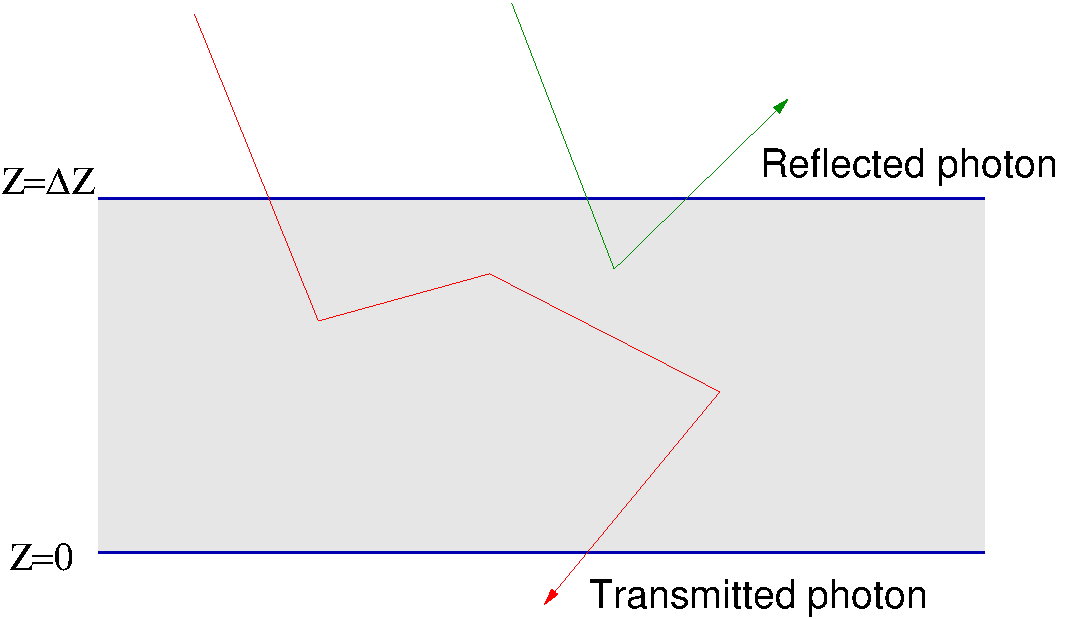
\includegraphics[width=0.8\hsize]{./figs/domain_cloudonly.pdf}
  \caption{Schematic of homogeneous horizontally infinite cloud
    layer.}
    \label{fig:cloudonly}
\end{figure}

\subsection{How to program a simple Monte Carlo model} 

In a Monte Carlo model a large number of photons are traced through
the model domain following probabilistic assumptions about the
interaction with the medium. The following steps are required to
describe the photon path:

\begin{enumerate}
\item Initialization: As position only the vertical coordinate $z$ is
  required since the medium is homogeneous and infinite in the
  horizontal. Starting point is the top of the cloud layer, $z=\Delta z$.
  The direction is given by the solar zenith angle $\theta_0$. 
  It is convenient to define a direction vector $\vec{dx}$.
\item Generate a random optical thickness $\tau$ and calculate the
  distance corresponding to this $\tau$ given the direction of the
  photon $\vec{dx}$ and the vertical optical thickness of the cloud
  $\tau_c$. Calculate the new position $z_p$ after the photon has
  traversed the optical thickness $\tau$.
\item Scattering: Calculate the direction of the photon after it is
  scattered. Suppose that the probability distribution of scattering angles
  $\mu$ is given by the Henyey-Greenstein phase function. In addition
  to $\mu$ a random azimuthal angle $\phi$ is required to calculate
  the new direction after the scattering process. 
\item Go back to step 2.
\item Repeat steps 2 and 3 until the photon reaches the top of the
  cloud layer or the bottom. Here count the photon. 
\end{enumerate}
Repeat this procedure for a large number of photons. Finally the
transmittance of the cloud layer is defined as
\begin{equation}
  T = \frac{N_{z=0}}{N_{tot}}\cos\theta_0
\end{equation}
and the reflectance is
\begin{equation}
  R = \frac{N_{z=\Delta z}}{N_{tot}}\cos\theta_0
\end{equation}
where $N_{tot}$ is the total number of photons, $N_{z=0}$ is the number of
photons counted at the bottom of the layer and $N_{z=\Delta z}$ is the
number of photons at the top of the layer. To calculate the irradiance
the transmittance/reflectance is just multiplied with the
extraterrestrial solar irradiance.  

The accuracy of the Monte Carlo method depends only on the number of
photons. If the number of photons is sufficiently large, it follows
from Gaussian statistics that the relative error (1$\sigma$) is given by:
\begin{equation}
  \label{eq:error}
  \sigma = \sqrt{\frac{N_{tot}-N}{N_{tot}N}}
\end{equation}
where $N$ is the number of counted photons for the quantity to be computed.

\subsection{Tasks}
\begin{enumerate}
\item Write a Monte Carlo code following the steps described above.
\item All photons must end up either at the top of the layer or at the
  bottom, otherwise your model would not fullfill energy
  conservation. Check whether $N_{z=0}+N_{z=\Delta z}=N_{tot}$.
\item Calculate transmittance and reflectance of the cloud layer using
  various different input values of $N_{tot}$,
  $\tau_c$, $\theta_0$ and $g$ and validate your model by comparing
  the results to the values in Table \ref{tab:cloudonly_result} 
  and to Fig.~\ref{fig:cloudonly_result}.
\end{enumerate}

\begin{figure}[htbp]
  \centering
  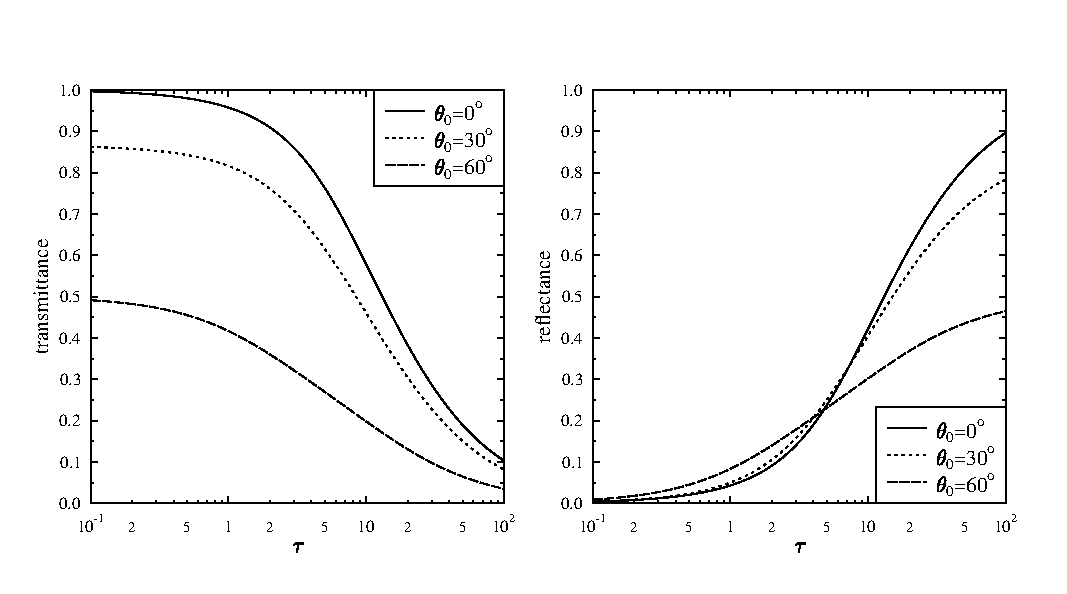
\includegraphics[width=1.\hsize]{./figs/plot_gg085_alb0.pdf}\\
  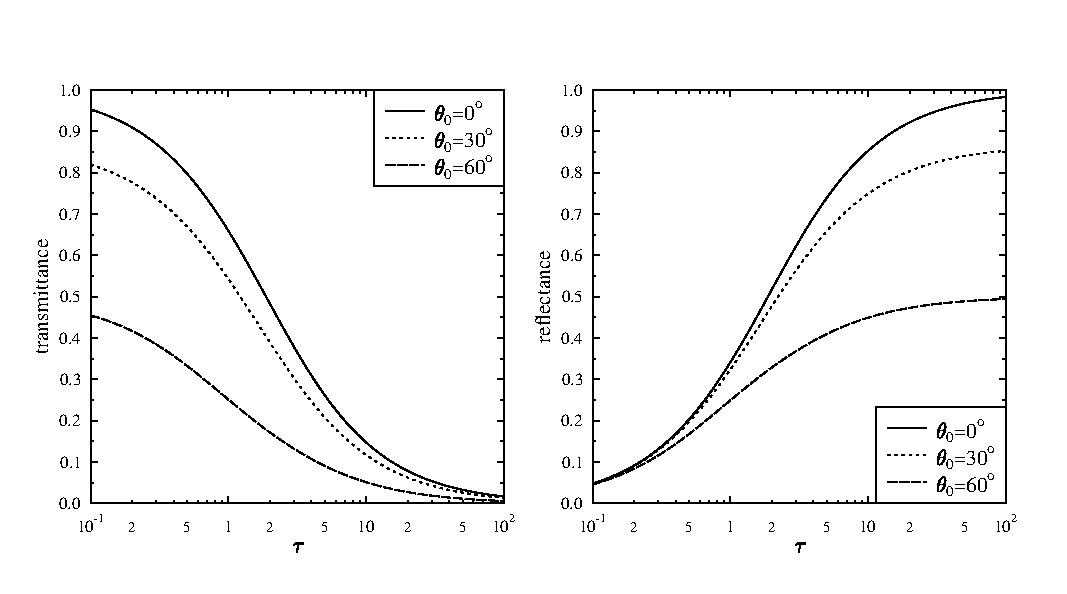
\includegraphics[width=1.\hsize]{./figs/plot_gg0_alb0.pdf}\\
  \caption{Reflectance and transmittance as a function of optical
    thickness. Different curves correspond to different solar zenith
    angles $\theta_0$. The top figures show the results for a
    Henyey-Greenstein phase function with an asymmetry parameter of
    $g=0.85$ and the bottom figures show the same calculation for
    isotropic scattering $g=0$. The results are computed using a
    discrete ordinate radiative transfer code (DISORT) which is one of
    the solvers implemented in the libRadtran radiative transfer
    package \citep{mayer2005}.}
    \label{fig:cloudonly_result}
\end{figure}


\begin{table*}
  \centering
  \begin{tabular}{c c c c}
    \hline
    optical thickness $\tau_c$ & solar zenith angle $\theta_0$ [ $^\circ$ ] & transmittance &
    reflectance \\ \hline
    1    &  0 & 0.957 & 0.043 \\
    10   &  0 & 0.578 & 0.422 \\ 
    100   &  0 & 0.103 & 0.897 \\
    1  & 30 & 0.816 & 0.050 \\
    10 & 30 & 0.460 & 0.406 \\
    100 & 30 & 0.082 & 0.784 \\
    1 & 60 & 0.417 & 0.084 \\
    10 & 60 & 0.198 & 0.302 \\
    100 & 60 & 0.035 &  0.465 \\ \hline
  \end{tabular}
  \caption{Transmittance and reflectance of a 1D cloud layer assuming
    a Henyey-Greenstein phase function with g=0.85.}
  \label{tab:cloudonly_result}
\end{table*}


\cleardoublepage
\section{Rayleigh scattering and gas absorption}
\label{sec:molecules}

\subsection{Setup: Cloudless sky Earth atmosphere}

The Earth's atmosphere consists of various gas species, e.g. N$_2$,
O$_2$, O$_3$ etc. Molecules are small compared to the wavelength of
solar radiation, hence they interact as Rayleigh scatterers.  
The number density of air molecules decreases exponentially with
height according to the hydrostatic equation. Therefore the clearsky
atmosphere can not be treated as a homogeneous medium. 
We may assume that the atmosphere consists of homogeneous
plane-parallel vertical layers (see Fig. \ref{fig:clear}).
For simplicity we assume that the surface absorbs all photons,
i.e. the surface albedo is 0. This is realistic for a water surface. 
Molecules interact with solar radiation by scattering and also by 
absorption. The extinction of a layer is given by
\begin{equation}
  \beta_\mathrm{ext}=\beta_\mathrm{sca}+\beta_\mathrm{abs}
\end{equation}
where $\beta_\mathrm{sca}$ is the volume scattering coefficient and
$\beta_\mathrm{abs}$ is the volume absorption coefficient. 


\begin{figure}[htbp]
  \centering
  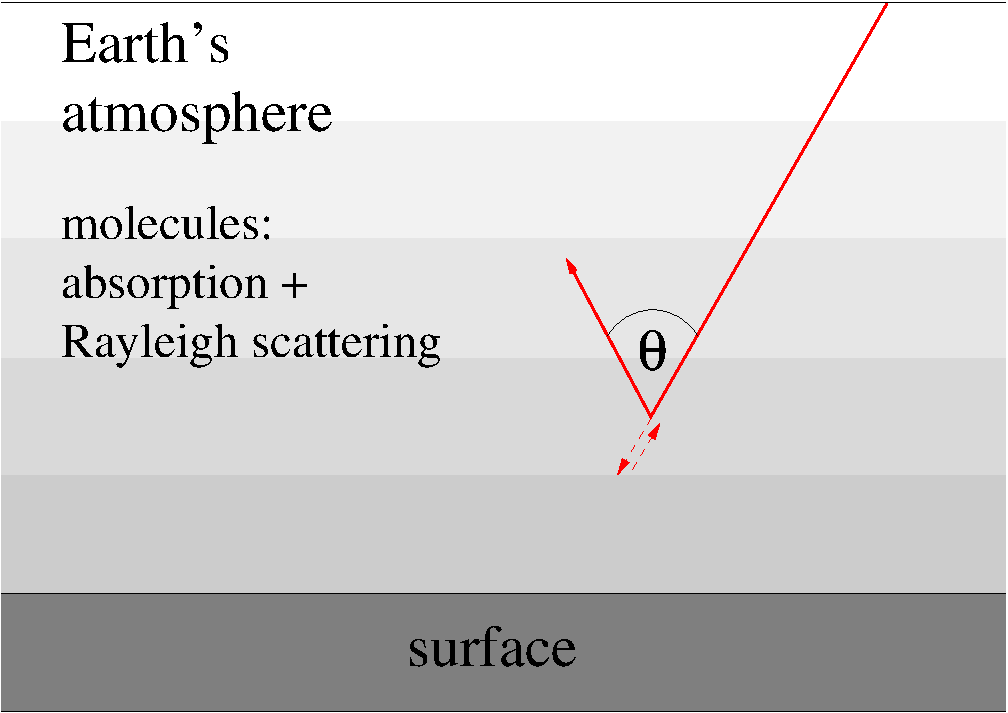
\includegraphics[width=0.8\hsize]{./figs/domain_clear.pdf}
  \caption{Schematic of cloudless Earth atmosphere.}
    \label{fig:clear}
\end{figure}

In order to obtain profiles of $\beta_\mathrm{sca}$ and $\beta_\mathrm{abs}$ one can
use reference atmospheres which contain profiles of
pressure, temperature and the constituent concentrations.
Several such reference atmospheres have been compiled by 
\citet{Anderson1986}. In addition the absorption cross sections of the
molecules are required. These can be obtained from databases, for
instance from the HITRAN database \citep{Rothman1987}. 

\subsection{Implementation of Rayleigh scattering}

In order to calculate the transmittance of a vertically inhomogeous
atmosphere, the model domain is devided into a discrete number of
plane-parallel layers. The implementation of Rayleigh scattering is
then very similar to the procedure described in section
\ref{sec:clouds}. The only differences are the scattering phase
function and the calculation of the free path of the photon. To sample
the scattering angle, of course we have to use the Rayleigh phase
function here. To calculate the free path corresponding to a randomly
sampled $\tau$, we have to go through the discrete layers step by step.

\subsection{Implementation of molecular absorption} 

When a photon interacts with a molecule by absorption, the molecule
uses the energy of the photon to be transfered to an activated state. For
a photon in the Monte Carlo Model this means that it
is eliminated immediately. One way to implement absorption is to
use the single scattering albedo
\begin{equation}
  \omega_0=\frac{\beta_\mathrm{sca}}{\beta_\mathrm{ext}}
\end{equation}
 $\omega_0$ is a number between 0 and 1; 0 means that
there is only absorption and 1 means that there is only
scattering. Now we may use a random number to decide whether the
photon interacts with the medium via scattering or via absorption. If
the random number is larger than $1-\omega_0$ the interaction is a
scattering event and else the photon is absorbed. 

A problem of this approach is that it is not very efficient. All
photons that are absorbed do not contribute to the result of the Monte
Carlo calculation and therefore the statistical error increases. 
To treat absorption in a  more efficient way we may assign a weight to each
photon. In the beginning the weight is 1 and absorption decreases the
weight but does not eliminate the photon. The weight $w_\mathrm{abs}$ of the photon
due to absorption is given by 
\begin{equation}
  \label{eq:weight}
  w_\mathrm{abs}=\exp(-\tau_\mathrm{abs})
\end{equation}
In this case we have to use the probability density function
\begin{equation}
   P(\tau_\mathrm{sca})=\exp(-\tau_\mathrm{sca}) 
\end{equation}
in order to sample the free pathlength of the photons.
Finally, when we sum up the photons to get the transmittance, we
calculate
\begin{equation}
  T=\frac{\sum_1^{N_{z=0}} w_i}{N_\mathrm{tot}} \cos\theta_0
\end{equation}

\subsection{Tasks}
\begin{enumerate}
\item Tables of pre-calculated $\beta_\mathrm{sca}$ and
  $\beta_\mathrm{abs}$ profiles are provided. The tables correspond to
  different wavelengths. Read these tables to define your
  model atmosphere.
\item Extend your photon tracing function to allow vertical
  inhomogeneous extinction and absorption coefficient profiles.
\item Sample random scattering angles according to the Rayleigh phase
  function.  
\item Implement molecular absorption using one of the methods
  described above (use single scattering albedo or assign a photon weight).
  If you have time implement both and compare the results.
\item Calculate the transmittance and reflectance for different 
  wavelenghts and various solar
  zenith angles and compare your results with
  Fig.~\ref{fig:rayleigh_result}
  and Table~\ref{tab:rayleigh_result}.  
\end{enumerate}

\begin{figure}[htbp]
  \centering
  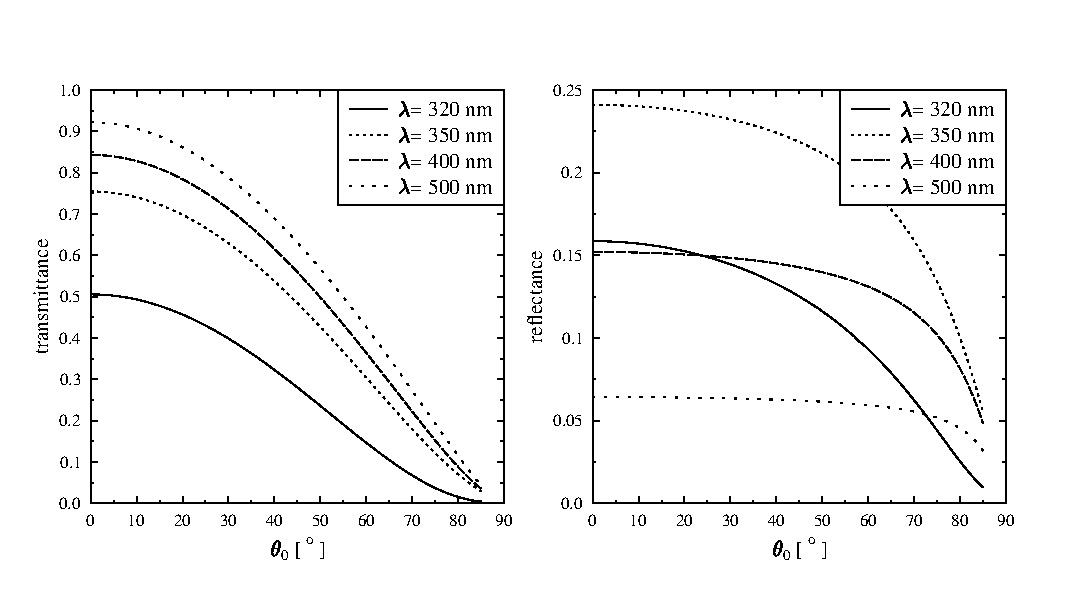
\includegraphics[width=1.\hsize]{./figs/rayleigh.pdf}\\
  \caption{Reflectance and transmittance of a typical Rayleigh
    atmosphere as a function of solar zenith
    angle. Different curves correspond to different wavelengths
    $\lambda$. The results are computed using a
    discrete ordinate radiative transfer code (DISORT) which is one of
    the solvers implemented in the libRadtran radiative transfer
    package \citep{mayer2005}.}
    \label{fig:rayleigh_result}

\end{figure}
\begin{table*}
  \centering
  \begin{tabular}{c c c c}
    \hline
    wavelength $\lambda$ [ nm ]  & solar zenith angle $\theta_0$ [ $^\circ$ ] & transmittance &
    reflectance \\ \hline
    320 & 0  & 0.505 & 0.159 \\
    350 &  0 & 0.755 & 0.241 \\
    400 &  0 & 0.843 & 0.152 \\ 
    500 &  0 & 0.922 & 0.064 \\
    320 & 30 & 0.397 & 0.145 \\
    350 & 30 & 0.621 & 0.232 \\
    400 & 30 & 0.712 & 0.148 \\
    500 & 30 & 0.788 & 0.063 \\
    320 & 60 & 0.147 & 0.096 \\
    350 & 60 & 0.304 & 0.192 \\
    400 & 60 & 0.364 & 0.131 \\
    500 & 60 & 0.427 & 0.059 \\ \hline
  \end{tabular}
  \caption{Transmittance and reflectance of a typical clearsky
    Rayleigh atmosphere.}
  \label{tab:rayleigh_result}
\end{table*}


\cleardoublepage

\section{Atmosphere with clouds and molecules} 

\subsection{Lambert surface} 

So far we have neglected reflection at the surface. We have
already discussed how to sample the direction of the reflection for a
Lambertian surface in section \ref{sec:surface}. 
To include surface reflection in the Monte Carlo model we may use
another random number $r$ when the photon hits the surface. If $r<a$,
where $a$ is the surface albedo, the photon is absorbed by the surface
and otherwise it is reflected.
Another more efficient method is to always reflect the photon at the
surface and to multiply the photon weight with the surface albedo.
 
\subsection{Rayleigh atmosphere with clouds}

In the real atmosphere there may be clouds and molecules at the
same time. Again we may use a random number $r$ to decide
whether the photon interacts with a cloud droplet or a molecule. 
If the random number is smaller than the ratio between the Rayleigh
scattering coefficient and the total scattering coefficient, 
the photon interacts with the molecule:
\begin{equation}
  r \le \frac{\beta_\mathrm{sca,r}}{\beta_\mathrm{sca,r}+\beta_\mathrm{sca,c}}
\end{equation}
Here $\beta_\mathrm{sca,r}$ is the Rayleigh scattering coefficient
and $\beta_\mathrm{sca,c}$ is the cloud scattering coefficient. Else,
if the random number is larger than this ratio the photon interacts
with the cloud droplet. 

\begin{figure}[htbp]
  \centering
  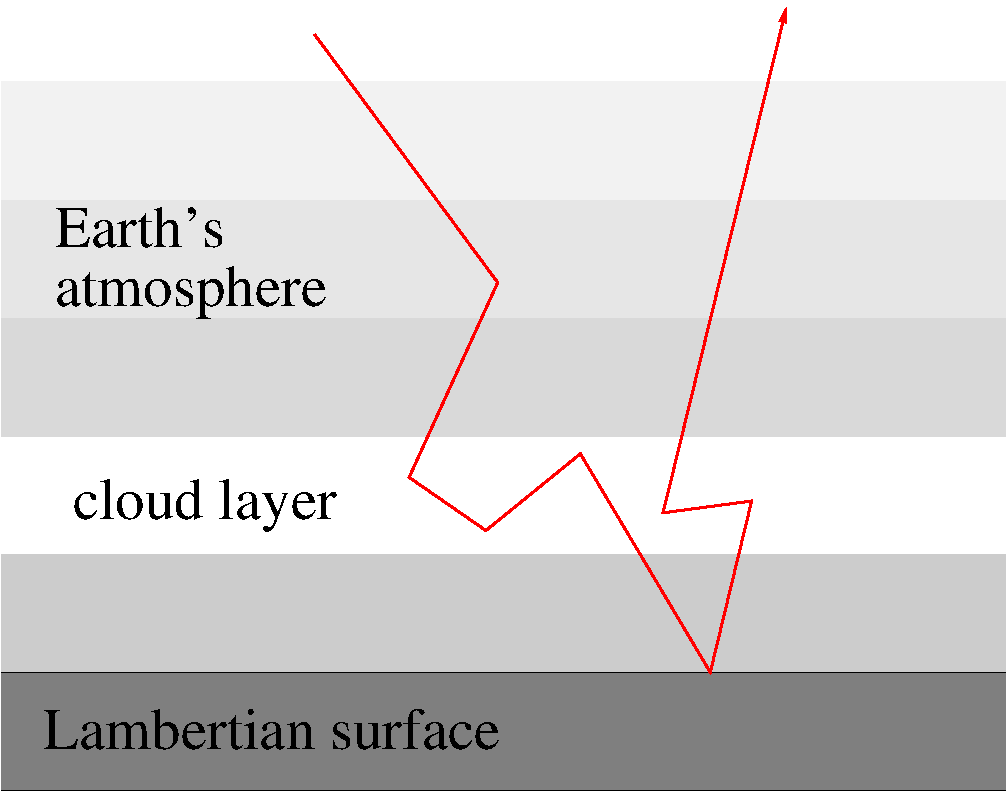
\includegraphics[width=0.8\hsize]{./figs/domain_cloudy.pdf}
  \caption{Schematic of a 1D-plane-parallel model with a 
    cloud layer and a Lambertian surface.} 
    \label{fig:cloudy}
\end{figure}

\subsection{Calculation of irradiance}
We have calculated the transmittance and reflectance of the
atmosphere. These quantities cannot be compared directly to the
measurements. A quantity that can be measured is the irradiance. It is
defined as the flow of radiative energy per unit area per wavelength.
The unit of
irradiance is W/(m$^2$ nm). To obtain the irradiance we just have to
multiply the transmittance and the reflectance with the
extraterrestrial irradiance (Fig.~\ref{fig:solar_spectrum}).

\begin{figure}[htbp]
  \centering
  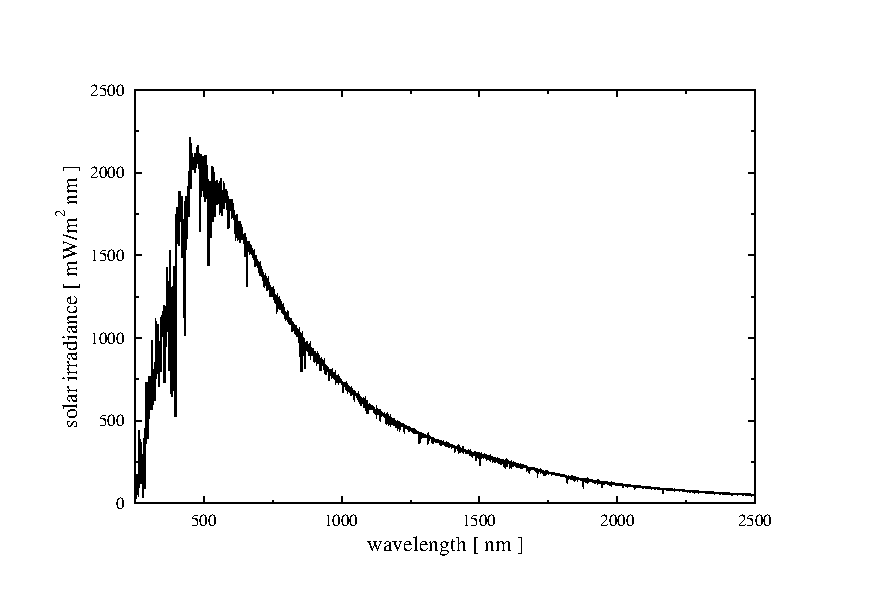
\includegraphics[width=1.\hsize]{./figs/kurutz.pdf}\\
  \caption{Extraterrestrial solar spectrum \citep{kurucz92}.}
  \label{fig:solar_spectrum}
\end{figure}


\subsection{Tasks}
\begin{enumerate}

\item Implement surface reflection assuming a Lambertian surface.
\item Calculate transmittance and reflectance for various surface
  albedos for a clearsky atmosphere and compare the results with 
  Fig.~\ref{fig:lambert}. 
\item Include a cloud layer in your model.
\item Compute transmittance and reflectance for the cloudy Earth
  atmosphere.
\item Multiply the transmittance and reflectance values with the
  extraterrestrial irradiance (Fig.~\ref{fig:solar_spectrum}) to
  obtain the radiative flux at the 
  surface and at the top of the atmosphere. 
 
\end{enumerate}
 
\begin{figure}[htbp]
  \centering
  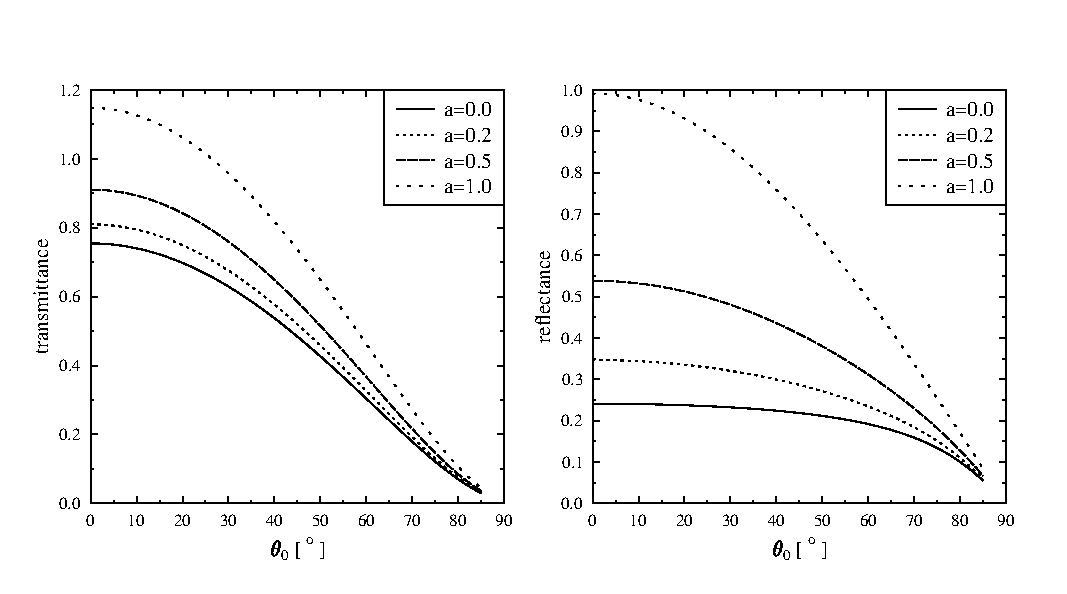
\includegraphics[width=1.0\hsize]{./figs/lambert.pdf}\\
  \caption{Transmittance and reflectance at a wavelength of 350 nm for
    as a function of solar zenith angle different surface
    albedos. The results are computed using the
    discrete ordinate radiative transfer code DISORT.}
  \label{fig:lambert}
\end{figure}

\cleardoublepage 

\section{Calculation of radiance}

\subsection{Cone sampling}

So far we have computed solar irradiances which in case of
transmittance include all photons reaching the surface no matter from
which direction. 
Another quantity that is frequently measured is the radiance. The
radiance is the flow of energy per unit area per unit solid angle. The
unit of radiance is W/(m$^2$ nm sr). A simple method to compute the
radiance is to sample photons into a cone centered around the desired
direction (see figure \ref{fig:cone}). 
\begin{figure}[htbp]
  \centering
  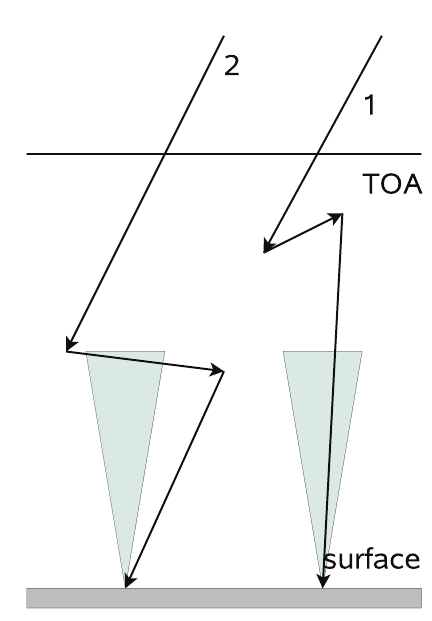
\includegraphics[width=0.4\hsize]{./figs/cone_sampling.png}\\
  \caption{Cone sampling to compute radiances (from
    \citet{mayer2009}). Photon 1 is counted whereas photon 2 misses
    the cone and does not contribute to the result.}
  \label{fig:cone}
\end{figure}
The problem with this method is that the probability that the photon
hits the cone is very very small. A second disadvantage is that we do
not really calculate the radiance in the desired direction, but an
average over the solid angle interval formed by the cone. 


\subsection{Local or directional estimate techniques}

A much more efficient method is the so-called local or directional
estimate technique \citep{mayer2009, marshak2005}. Here we calculate
at each scattering point the probability that the photon is scattered
into the direction of the sensor (see figure \ref{fig:loc_est}). Note that the actual photon path is
not affected by this technique. 
\begin{figure}[htbp]
  \centering
  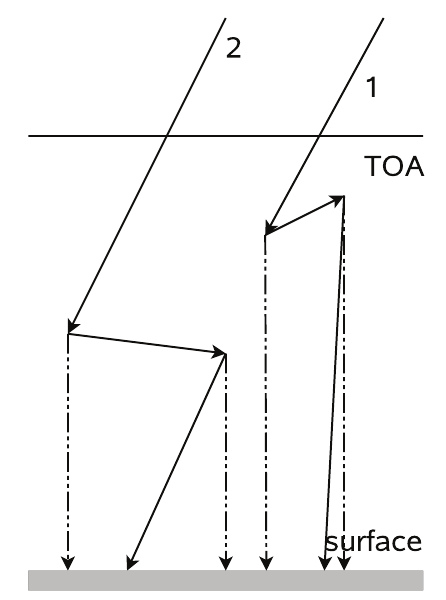
\includegraphics[width=0.4\hsize]{./figs/local_estimate.png}\\
  \caption{The local/directional estimate technique (from
    \citet{mayer2009}).}
  \label{fig:loc_est}
\end{figure}
The probability for scattering into
the direction of the sensor is given by the phase function taking into
account the extinction between scattering and detector. In order to
compute the radiance, we just sum up the following weights calculated
at each scattering point: 
\begin{equation}
  w=w_0 \cdot P(\theta_p) \cdot \exp(-\tau_\mathrm{ext}) / \cos(\theta_d)
\end{equation}
where $w_0$ is the photon weight (which includes absorption and may be
also the surface reflection). $\theta_p$ is the angle between photon
direction (before scattering) and the radiance direction. The phase
function $P(\theta_p)$ gives the probability that the photon is
scattered into the direction of the detector. To calculate the
probability that the photon actually reaches the detector the
Lambert-Beer term for extinction $ \exp(-\tau_\mathrm{ext})$ needs to
be included. We need to devide by the zenith angle of the detector
direction $\theta_d$ to account for the slant area in the definition of
the radiance. The same needs to be done when a photon hits the
surface, using the albedo for the photon weight instead of the
scattering phase function. 
Using this method each photon contributes several times to the
radiances. 

\subsection{Tasks}

\begin{enumerate}
\item Implement the local estimate technique to compute radiances.
\item Perform calculations for various setups (clear-sky atmosphere,
  cloudy atmosphere, different surface albedo).
\item Investigate the contributions of individual scattering orders to
  the result. 
\end{enumerate}


%\cleardoublepage


\clearpage

%% bibliography
%\addcontentsline{toc}{chapter}{Bibliography}
%\markright{BIBLIOGRAPHY}
\bibliography{/home/claudia/bibtex/literature}
%\bibliography{/home/users/emde/bibtex/literature}

\end{document}

 
